\documentclass[tikz,border=4pt]{standalone}
\usepackage{amsmath}
\definecolor{curveblue}{HTML}{245C86}
\begin{document}
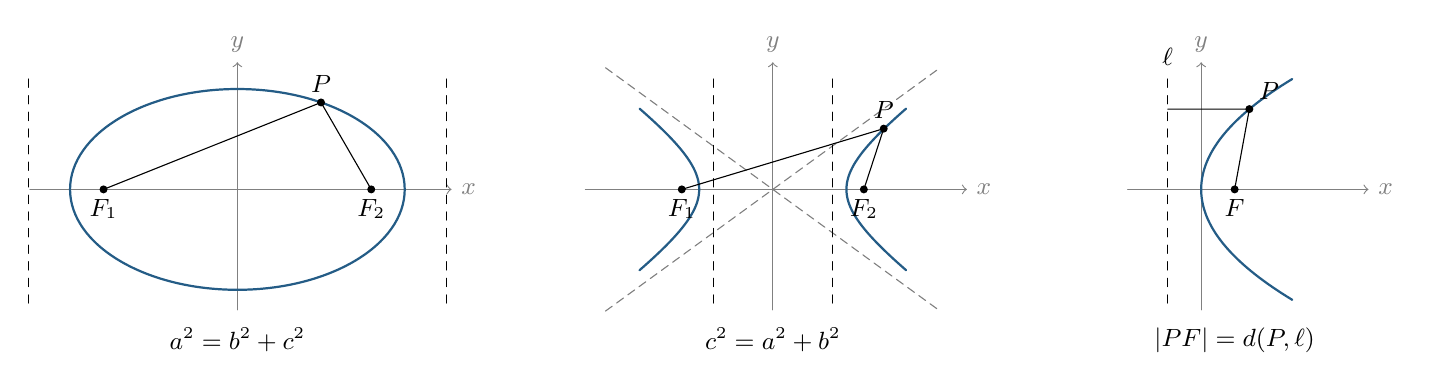
\begin{tikzpicture}[line cap=round,font=\small,scale=.85]
\begin{scope}
\draw[->,gray](-3.1,0)--(3.2,0)node[right]{$x$};
\draw[->,gray](0,-1.8)--(0,1.9)node[above]{$y$};
\draw[curveblue,thick](0,0)ellipse[x radius=2.5,y radius=1.5];
\draw[dashed](-3.125,-1.7)--(-3.125,1.7) (3.125,-1.7)--(3.125,1.7);
\fill(-2,0)circle(1.7pt)node[below]{$F_1$};
\fill(2,0)circle(1.7pt)node[below]{$F_2$};
\coordinate(P)at(1.25,1.299);
\draw(-2,0)--(P)--(2,0);\fill(P)circle(1.7pt)node[above]{$P$};
\node at(0,-2.25){$a^2=b^2+c^2$};
\end{scope}
\begin{scope}[shift={(8,0)}]
\draw[->,gray](-2.8,0)--(2.9,0)node[right]{$x$};
\draw[->,gray](0,-1.8)--(0,1.9)node[above]{$y$};
\draw[gray,densely dashed](-2.5,-1.818)--(2.5,1.818) (-2.5,1.818)--(2.5,-1.818);
\draw[curveblue,thick,domain=-1.2:1.2,samples=60]plot({1.1*cosh(\x)},{.8*sinh(\x)});
\draw[curveblue,thick,domain=-1.2:1.2,samples=60]plot({-1.1*cosh(\x)},{.8*sinh(\x)});
\draw[dashed](-.8895,-1.7)--(-.8895,1.7) (.8895,-1.7)--(.8895,1.7);
\fill(-1.3601,0)circle(1.7pt)node[below]{$F_1$};
\fill(1.3601,0)circle(1.7pt)node[below]{$F_2$};
\coordinate(P)at(1.657, .908);
\draw(-1.3601,0)--(P)--(1.3601,0);\fill(P)circle(1.7pt)node[above]{$P$};
\node at(0,-2.25){$c^2=a^2+b^2$};
\end{scope}
\begin{scope}[shift={(14.4,0)}]
\draw[->,gray](-1.1,0)--(2.5,0)node[right]{$x$};
\draw[->,gray](0,-1.8)--(0,1.9)node[above]{$y$};
\draw[curveblue,thick,domain=-1.65:1.65,samples=70]plot({\x*\x/2},{\x});
\draw[dashed](-.5,-1.7)--(-.5,1.7)node[above]{$\ell$};
\fill(.5,0)circle(1.7pt)node[below]{$F$};
\coordinate(P)at(.72,1.2);\draw(.5,0)--(P)--(-.5,1.2);
\fill(P)circle(1.7pt)node[above right]{$P$};
\node at(.5,-2.25){$|PF|=d(P,\ell)$};
\end{scope}
\end{tikzpicture}
\end{document}
